\documentclass[11pt]{article}

\usepackage[a4paper,margin=1in]{geometry}
\usepackage[T1]{fontenc}
\usepackage[utf8]{inputenc}
\usepackage{lmodern}
\usepackage{amsmath,amssymb,amsthm,mathtools,bm}
\usepackage{graphicx}
\usepackage{booktabs}
\usepackage{array}
\usepackage{enumitem}
\usepackage{microtype}
\usepackage{xcolor}
\usepackage{hyperref}
\usepackage{caption}
\usepackage{float}
\usepackage{setspace}
\usepackage{fancyhdr}

\hypersetup{
  colorlinks=true,
  linkcolor=blue!50!black,
  citecolor=blue!50!black,
  urlcolor=blue!50!black,
  pdftitle={Laplace AR(1) under OU corruption: detailed derivation note},
  pdfauthor={OpenAI}
}

\setlength{\headheight}{14pt}
\pagestyle{fancy}
\fancyhf{}
\lhead{Laplace AR(1) under OU corruption}
\rhead{Detailed derivation note}
\cfoot{\thepage}

\setstretch{1.08}
\setlength{\parskip}{0.35em}
\setlength{\parindent}{0pt}

\newcommand{\R}{\mathbb{R}}
\newcommand{\E}{\mathbb{E}}
\newcommand{\Var}{\operatorname{Var}}
\newcommand{\Cov}{\operatorname{Cov}}
\newcommand{\diag}{\operatorname{diag}}
\newcommand{\tr}{\operatorname{tr}}
\newcommand{\sgn}{\operatorname{sgn}}
\newcommand{\dd}{\mathrm{d}}
\newcommand{\e}{\mathrm{e}}
\newcommand{\ii}{\mathrm{i}}
\newcommand{\1}{\mathbf{1}}
\newcommand{\trans}{^{\mathsf T}}
\newcommand{\pt}{p_t}
\newcommand{\ph}{\varphi}
\newcommand{\Ph}{\Phi}
\newcommand{\score}{\mathcal{S}}
\newcommand{\curv}{\mathcal{H}}
\newcommand{\NL}{\mathrm{NL}}
\newcommand{\Laplace}{\mathrm{Laplace}}
\newcommand{\Normal}{\mathcal{N}}
\newcommand{\given}{\,|\,}
\newcommand{\br}[1]{\left(#1\right)}
\newcommand{\sq}[1]{\left[#1\right]}
\newcommand{\cb}[1]{\left\{#1\right\}}
\newcommand{\abs}[1]{\left|#1\right|}
\newcommand{\norm}[1]{\left\lVert #1 \right\rVert}
\newcommand{\gauss}[2]{\frac{1}{\sqrt{2\pi #2}}\exp\!\left(-\frac{#1^2}{2#2}\right)}

\theoremstyle{definition}
\newtheorem{remark}{Remark}
\newtheorem{proposition}{Proposition}
\newtheorem{lemma}{Lemma}

\begin{document}

\begin{center}
    {\LARGE \textbf{Laplace AR(1) under Ornstein--Uhlenbeck Corruption}}\\[0.4em]
    {\large A detailed derivation note for the score, the residual representation, the Fourier picture, and the curvature field}\\[1em]
    {\normalsize This note is written to be editable: every symbol is defined, every transformation is shown, and the key formulas are isolated so they can be modified easily.}
\end{center}

\tableofcontents
\vspace{0.5em}

\section{Roadmap}

We study the scalar AR(1) model with Laplace innovation,
\begin{equation}
A_0 \sim \Normal(\mu_0,\sigma_0^2),
\qquad
A_1 = \alpha A_0 + \varepsilon,
\qquad
\varepsilon \sim \Laplace(0,b),
\end{equation}
with independent coordinates at the clean level:
\begin{equation}
\varepsilon \perp A_0.
\end{equation}

The observed noisy variables are generated through the Ornstein--Uhlenbeck (OU) channel
\begin{equation}
X_k = \beta A_k + \sqrt{\Delta}\, Z_k,
\qquad
\beta = \e^{-t},
\qquad
\Delta = 1-\e^{-2t}=1-\beta^2,
\qquad
Z_0,Z_1 \stackrel{\mathrm{i.i.d.}}{\sim} \Normal(0,1).
\end{equation}

We want explicit formulas for
\begin{equation}
\pt(x_0,x_1),
\qquad
\score(x,t)=\nabla_x \log \pt(x),
\qquad
\curv_t(x)=-\nabla_x^2 \log \pt(x).
\end{equation}

The central message is the following.

\medskip
\fbox{%
\parbox{0.94\linewidth}{%
For \(K=1\), the whole two-dimensional problem collapses to one Gaussian site variable \(x_0\) and one non-Gaussian residual variable
\[
r = x_1 - \nu - \rho x_0.
\]
The joint law factors as
\[
\pt(x_0,x_1)=\text{Gaussian in }x_0 \times \text{Normal--Laplace in }r,
\]
and the full Hessian field is controlled by a single scalar function
\[
\kappa_t(r) = -\frac{\dd^2}{\dd r^2}\log h_t(r),
\]
where \(h_t\) is the density of a Gaussian plus a scaled Laplace random variable.
}%
}
\medskip

Everything that looks two-dimensional in the heatmaps is therefore the image of a one-dimensional residual geometry transported along straight lines \(r=\mathrm{constant}\).

\section{Model, notation, and baseline densities}

\subsection{Clean density}

The Laplace density with location \(0\) and scale \(b>0\) is
\begin{equation}
\label{eq:laplace-density}
f_{\varepsilon}(u)=\frac{1}{2b}\exp\!\left(-\frac{|u|}{b}\right).
\end{equation}
Therefore the clean joint density of \((A_0,A_1)\) is
\begin{equation}
\label{eq:clean-joint-density}
p_0(a_0,a_1)
=
\frac{1}{\sqrt{2\pi\sigma_0^2}}
\exp\!\left(-\frac{(a_0-\mu_0)^2}{2\sigma_0^2}\right)
\cdot
\frac{1}{2b}\exp\!\left(-\frac{|a_1-\alpha a_0|}{b}\right).
\end{equation}

This formula already shows the clean geometry:
\begin{itemize}[leftmargin=2em]
    \item the \emph{root channel} \(a_0\) is Gaussian;
    \item the \emph{innovation channel} \(a_1-\alpha a_0\) is Laplace;
    \item the non-Gaussianity is concentrated on the bond variable \(a_1-\alpha a_0\).
\end{itemize}

\subsection{Noisy density as a Gaussian channel mixture}

Conditionally on \(A=(A_0,A_1)\), the noisy law is Gaussian with independent coordinates:
\begin{equation}
\label{eq:ou-kernel}
g_t(x|a)
=
\frac{1}{2\pi\Delta}
\exp\!\left(-\frac{(x_0-\beta a_0)^2+(x_1-\beta a_1)^2}{2\Delta}\right).
\end{equation}
Hence the noisy density is
\begin{equation}
\label{eq:noisy-integral}
\pt(x_0,x_1)=\int_{\R^2} g_t(x|a)\, p_0(a_0,a_1)\, \dd a_0\,\dd a_1.
\end{equation}

Because the clean law is Markov and the channel is coordinatewise conditionally independent, the noisy law preserves a one-step factorization:
\begin{equation}
\label{eq:markov-factorization-noisy}
\pt(x_0,x_1)=\pt(x_0)\,\pt(x_1\given x_0).
\end{equation}
Therefore the score is automatically local in the Markov sense:
\begin{equation}
\label{eq:score-markov-factorization}
\score(x,t)
=
\begin{pmatrix}
\partial_{x_0}\log \pt(x_0) + \partial_{x_0}\log \pt(x_1\given x_0)\\[0.6em]
\partial_{x_1}\log \pt(x_1\given x_0)
\end{pmatrix}.
\end{equation}

Equation \eqref{eq:score-markov-factorization} is the first exact locality statement. The second component depends only on the single edge potential \(\pt(x_1\given x_0)\); the first component is a sum of one site term and one edge correction.

\section{The \(x_0\)-marginal and the posterior law of \(A_0\given X_0\)}

Since
\begin{equation}
X_0 = \beta A_0 + \sqrt{\Delta} Z_0,
\qquad
A_0\sim \Normal(\mu_0,\sigma_0^2),
\qquad
Z_0\sim \Normal(0,1),
\end{equation}
we immediately obtain
\begin{equation}
\label{eq:v-definition}
X_0\sim \Normal(\beta\mu_0,v),
\qquad
v := \beta^2 \sigma_0^2 + \Delta.
\end{equation}
Thus
\begin{equation}
\label{eq:px0}
\pt(x_0)=\frac{1}{\sqrt{2\pi v}}\exp\!\left(-\frac{(x_0-\beta\mu_0)^2}{2v}\right),
\end{equation}
and the corresponding marginal score is
\begin{equation}
\label{eq:px0-score}
\partial_{x_0}\log \pt(x_0) = -\frac{x_0-\beta\mu_0}{v}.
\end{equation}

Now compute the posterior law of \(A_0\given X_0=x_0\). Since everything is jointly Gaussian, it is again Gaussian. The standard conditioning formulas give
\begin{equation}
\label{eq:posterior-A0-X0}
A_0\given X_0=x_0 \sim \Normal\big(m(x_0),s^2\big),
\end{equation}
with
\begin{equation}
\label{eq:m-s-definitions}
m(x_0)=\mu_0 + \frac{\Cov(A_0,X_0)}{\Var(X_0)}(x_0-\beta\mu_0),
\qquad
s^2 = \Var(A_0)-\frac{\Cov(A_0,X_0)^2}{\Var(X_0)}.
\end{equation}
Because
\begin{equation}
\Cov(A_0,X_0)=\Cov(A_0,\beta A_0 + \sqrt{\Delta}Z_0)=\beta\sigma_0^2,
\end{equation}
we obtain
\begin{equation}
\label{eq:m-explicit}
m(x_0)=\mu_0 + \frac{\beta\sigma_0^2}{v}(x_0-\beta\mu_0)
=\frac{\Delta\mu_0+\beta\sigma_0^2 x_0}{v},
\end{equation}
and
\begin{equation}
\label{eq:s2-explicit}
s^2 = \sigma_0^2 - \frac{\beta^2\sigma_0^4}{v}
=\frac{\sigma_0^2\Delta}{v}.
\end{equation}

These two quantities are fundamental. The noisy root variable \(X_0\) carries all available information about \(A_0\), and all remaining uncertainty is contained in the posterior variance \(s^2\).

\section{Conditional law of \(X_1\given X_0=x_0\): reduction to one residual variable}

The next task is to compute \(\pt(x_1\given x_0)\). Start from
\begin{equation}
X_1 = \beta A_1 + \sqrt{\Delta} Z_1 = \beta(\alpha A_0 + \varepsilon)+\sqrt{\Delta} Z_1.
\end{equation}
Insert the decomposition
\begin{equation}
A_0 = m(x_0)+\xi,
\qquad
\xi\given X_0=x_0 \sim \Normal(0,s^2),
\qquad
\xi \perp (X_0,\varepsilon,Z_1).
\end{equation}
Then
\begin{align}
X_1
&= \beta\alpha m(x_0) + \beta\alpha\xi + \beta\varepsilon + \sqrt{\Delta}Z_1 \\
&= \beta\alpha m(x_0) + \beta\varepsilon + G_t,
\end{align}
where
\begin{equation}
\label{eq:Gt-definition}
G_t := \beta\alpha\xi + \sqrt{\Delta}Z_1 \sim \Normal(0,\tau^2),
\end{equation}
with variance
\begin{equation}
\label{eq:tau2-definition}
\tau^2 = \beta^2\alpha^2 s^2 + \Delta
= \Delta + \alpha^2\beta^2\frac{\sigma_0^2\Delta}{v}.
\end{equation}

We now isolate the \(x_0\)-dependence of the mean term:
\begin{equation}
\beta\alpha m(x_0)=\nu + \rho x_0,
\end{equation}
with
\begin{equation}
\label{eq:rho-nu-definitions}
\rho := \alpha\frac{\beta^2\sigma_0^2}{v},
\qquad
\nu := \alpha\beta\frac{\Delta\mu_0}{v}.
\end{equation}
Indeed, substituting \eqref{eq:m-explicit} gives
\begin{equation}
\beta\alpha m(x_0)=\beta\alpha\frac{\Delta\mu_0+\beta\sigma_0^2 x_0}{v}
=\alpha\beta\frac{\Delta\mu_0}{v} + \alpha\frac{\beta^2\sigma_0^2}{v}x_0.
\end{equation}

Therefore
\begin{equation}
\label{eq:X1-cond-structure}
X_1\given X_0=x_0 = \nu + \rho x_0 + R_t,
\end{equation}
where the residual variable is
\begin{equation}
\label{eq:Rt-definition}
R_t := \beta\varepsilon + G_t,
\qquad
G_t\sim \Normal(0,\tau^2),
\qquad
R_t \perp X_0.
\end{equation}

This is the main structural reduction. The entire non-Gaussian problem is now encoded in the one-dimensional random variable \(R_t\), which is a Gaussian plus a scaled Laplace variable.

\subsection{Exact factorized form of the joint density}

Let \(h_t\) denote the density of \(R_t\). Then \eqref{eq:X1-cond-structure} implies
\begin{equation}
\label{eq:conditional-density-via-residual}
\pt(x_1\given x_0)=h_t\big(x_1-\nu-\rho x_0\big).
\end{equation}
Combining this with \eqref{eq:px0} yields the exact joint density
\begin{equation}
\label{eq:joint-factorized-final}
\boxed{
\pt(x_0,x_1)=\frac{1}{\sqrt{2\pi v}}\exp\!\left(-\frac{(x_0-\beta\mu_0)^2}{2v}\right)\, h_t(r),
\qquad
r:=x_1-\nu-\rho x_0.
}
\end{equation}

From this point onward, every derivative can be computed by the chain rule from a one-dimensional function \(h_t\).

\section{Derivation of the Normal--Laplace density \(h_t\)}

By construction,
\begin{equation}
\label{eq:ht-convolution}
h_t(r)=\int_{\R}\frac{1}{2\tilde b}\exp\!\left(-\frac{|u|}{\tilde b}\right)
\cdot
\frac{1}{\sqrt{2\pi\tau^2}}\exp\!\left(-\frac{(r-u)^2}{2\tau^2}\right)\dd u,
\end{equation}
where
\begin{equation}
\tilde b := \beta b.
\end{equation}

We now compute this integral explicitly. Split the real line into positive and negative parts:
\begin{equation}
\label{eq:ht-split}
h_t(r)=\frac{1}{2\tilde b\sqrt{2\pi\tau^2}}
\left[
\int_0^{\infty} \exp\!\left(-\frac{u}{\tilde b}-\frac{(r-u)^2}{2\tau^2}\right)\dd u
+
\int_{-\infty}^{0} \exp\!\left(\frac{u}{\tilde b}-\frac{(r-u)^2}{2\tau^2}\right)\dd u
\right].
\end{equation}

\subsection{First integral: \(u\ge 0\)}

Consider
\begin{equation}
I_+(r):=\int_0^{\infty} \exp\!\left(-\frac{u}{\tilde b}-\frac{(r-u)^2}{2\tau^2}\right)\dd u.
\end{equation}
Expand the exponent and complete the square in \(u\):
\begin{align}
-\frac{u}{\tilde b}-\frac{(r-u)^2}{2\tau^2}
&= -\frac{u}{\tilde b} - \frac{u^2-2ru+r^2}{2\tau^2} \\
&= -\frac{u^2}{2\tau^2} + \left(\frac{r}{\tau^2}-\frac{1}{\tilde b}\right)u - \frac{r^2}{2\tau^2}.
\end{align}
Now write
\begin{equation}
\frac{r}{\tau^2}-\frac{1}{\tilde b} = \frac{r-\tau^2/\tilde b}{\tau^2},
\end{equation}
so
\begin{align}
-\frac{u^2}{2\tau^2} + \frac{r-\tau^2/\tilde b}{\tau^2}u
&= -\frac{1}{2\tau^2}\left[u^2 - 2(r-\tau^2/\tilde b)u\right] \\
&= -\frac{1}{2\tau^2}\left[(u-r+\tau^2/\tilde b)^2 - (r-\tau^2/\tilde b)^2\right].
\end{align}
Hence
\begin{align}
-\frac{u}{\tilde b}-\frac{(r-u)^2}{2\tau^2}
&= -\frac{(u-r+\tau^2/\tilde b)^2}{2\tau^2}
+ \frac{(r-\tau^2/\tilde b)^2-r^2}{2\tau^2} \\
&= -\frac{(u-r+\tau^2/\tilde b)^2}{2\tau^2} - \frac{r}{\tilde b} + \frac{\tau^2}{2\tilde b^2}.
\end{align}
Therefore
\begin{equation}
I_+(r)=\exp\!\left(-\frac{r}{\tilde b}+\frac{\tau^2}{2\tilde b^2}\right)
\int_0^{\infty}
\exp\!\left(-\frac{(u-r+\tau^2/\tilde b)^2}{2\tau^2}\right)
\dd u.
\end{equation}
Now use the substitution
\begin{equation}
z=\frac{u-r+\tau^2/\tilde b}{\tau},
\qquad
\dd u = \tau\,\dd z,
\qquad
u=0 \Longrightarrow z = -\frac{r}{\tau}+\frac{\tau}{\tilde b}.
\end{equation}
Then
\begin{align}
I_+(r)
&= \exp\!\left(-\frac{r}{\tilde b}+\frac{\tau^2}{2\tilde b^2}\right)
\tau\int_{-r/\tau+\tau/\tilde b}^{\infty} \exp\!\left(-\frac{z^2}{2}\right)\dd z \\
&= \exp\!\left(-\frac{r}{\tilde b}+\frac{\tau^2}{2\tilde b^2}\right)
\tau\sqrt{2\pi}\, \Ph\!\left(\frac{r}{\tau}-\frac{\tau}{\tilde b}\right).
\end{align}

\subsection{Second integral: \(u\le 0\)}

Similarly define
\begin{equation}
I_-(r):=\int_{-\infty}^{0} \exp\!\left(\frac{u}{\tilde b}-\frac{(r-u)^2}{2\tau^2}\right)\dd u.
\end{equation}
Complete the square again:
\begin{align}
\frac{u}{\tilde b}-\frac{(r-u)^2}{2\tau^2}
&= -\frac{u^2}{2\tau^2}+\left(\frac{r}{\tau^2}+\frac{1}{\tilde b}\right)u-\frac{r^2}{2\tau^2} \\
&= -\frac{(u-r-\tau^2/\tilde b)^2}{2\tau^2} + \frac{r}{\tilde b}+\frac{\tau^2}{2\tilde b^2}.
\end{align}
Therefore
\begin{equation}
I_-(r)=\exp\!\left(\frac{r}{\tilde b}+\frac{\tau^2}{2\tilde b^2}\right)
\int_{-\infty}^{0}
\exp\!\left(-\frac{(u-r-\tau^2/\tilde b)^2}{2\tau^2}\right)
\dd u.
\end{equation}
With the substitution
\begin{equation}
z=\frac{u-r-\tau^2/\tilde b}{\tau},
\qquad
u=0 \Longrightarrow z = -\frac{r}{\tau}-\frac{\tau}{\tilde b},
\end{equation}
we obtain
\begin{align}
I_-(r)
&= \exp\!\left(\frac{r}{\tilde b}+\frac{\tau^2}{2\tilde b^2}\right)
\tau\int_{-\infty}^{-r/\tau-\tau/\tilde b}\exp\!\left(-\frac{z^2}{2}\right)\dd z \\
&= \exp\!\left(\frac{r}{\tilde b}+\frac{\tau^2}{2\tilde b^2}\right)
\tau\sqrt{2\pi}\, \Ph\!\left(-\frac{r}{\tau}-\frac{\tau}{\tilde b}\right).
\end{align}

\subsection{Closed form}

Insert the two formulas into \eqref{eq:ht-split}. The factors \(\tau\sqrt{2\pi}\) cancel the Gaussian normalization, giving
\begin{equation}
\label{eq:ht-closed-form}
\boxed{
h_t(r)=\frac{\exp(a^2/2)}{2\tilde b}
\left[
\exp\!\left(-\frac{r}{\tilde b}\right)\Ph\!\left(\frac{r}{\tau}-a\right)
+
\exp\!\left(\frac{r}{\tilde b}\right)\Ph\!\left(-\frac{r}{\tau}-a\right)
\right],
\qquad
a:=\frac{\tau}{\tilde b}.
}
\end{equation}

This is the exact density of a Gaussian plus a scaled Laplace variable, often called the \emph{Normal--Laplace} law.

\section{Free energy form of the noisy law}

Using \eqref{eq:joint-factorized-final}, the log-density is
\begin{equation}
\label{eq:log-pt}
\log \pt(x_0,x_1)
=
-\frac{(x_0-\beta\mu_0)^2}{2v} + \log h_t(r) + \text{const}.
\end{equation}
Hence the negative log-density (free energy) is
\begin{equation}
\label{eq:free-energy}
F_t(x_0,x_1):=-\log \pt(x_0,x_1)
=
\frac{(x_0-\beta\mu_0)^2}{2v} + U_t(r) + \text{const},
\qquad
U_t(r):=-\log h_t(r).
\end{equation}

This decomposition is very important conceptually:
\begin{itemize}[leftmargin=2em]
    \item the term \(\frac{(x_0-\beta\mu_0)^2}{2v}\) is a quadratic site energy;
    \item the term \(U_t(r)\) is a bond energy depending on one residual variable only;
    \item Gaussianity is equivalent to \(U_t\) being quadratic;
    \item non-Gaussianity appears exactly as non-quadratic residual geometry.
\end{itemize}

\section{Score: exact formulas and nonlinear structure}

Define the residual score
\begin{equation}
\label{eq:psi-definition}
\psi_t(r):=\frac{\dd}{\dd r}\log h_t(r)=\frac{h_t'(r)}{h_t(r)}.
\end{equation}
Then from \eqref{eq:log-pt} and the chain rule
\begin{equation}
\partial_{x_1}r=1,
\qquad
\partial_{x_0}r=-\rho.
\end{equation}
Therefore
\begin{equation}
\label{eq:score-final}
\boxed{
\score(x,t)=
\begin{pmatrix}
-\dfrac{x_0-\beta\mu_0}{v} - \rho\, \psi_t(r)\\[0.8em]
\psi_t(r)
\end{pmatrix}.
}
\end{equation}

This formula cleanly separates the contributions:
\begin{itemize}[leftmargin=2em]
    \item \( -(x_0-\beta\mu_0)/v \): Gaussian root contribution;
    \item \( \psi_t(r) \): nonlinear innovation contribution;
    \item \( -\rho\psi_t(r) \): feedback of the bond onto the root score.
\end{itemize}

\subsection{Explicit formula for \(\psi_t\)}

Introduce
\begin{equation}
L_+(r):=\exp\!\left(-\frac{r}{\tilde b}\right)\Ph\!\left(\frac{r}{\tau}-a\right),
\qquad
L_-(r):=\exp\!\left(\frac{r}{\tilde b}\right)\Ph\!\left(-\frac{r}{\tau}-a\right),
\qquad a=\frac{\tau}{\tilde b}.
\end{equation}
Then \eqref{eq:ht-closed-form} becomes
\begin{equation}
h_t(r)=\frac{\exp(a^2/2)}{2\tilde b}\big(L_+(r)+L_-(r)\big).
\end{equation}
Differentiate term by term:
\begin{align}
L_+'(r)
&= -\frac{1}{\tilde b}L_+(r)+\frac{1}{\tau}\exp\!\left(-\frac{r}{\tilde b}\right)\ph\!\left(\frac{r}{\tau}-a\right),\\[0.5em]
L_-'(r)
&= \frac{1}{\tilde b}L_-(r)-\frac{1}{\tau}\exp\!\left(\frac{r}{\tilde b}\right)\ph\!\left(\frac{r}{\tau}+a\right).
\end{align}
Now use the identity
\begin{equation}
\exp\!\left(-\frac{r}{\tilde b}\right)\ph\!\left(\frac{r}{\tau}-a\right)
=
\exp\!\left(\frac{r}{\tilde b}\right)\ph\!\left(\frac{r}{\tau}+a\right)
=
\exp\!\left(-\frac{a^2}{2}\right)\ph\!\left(\frac{r}{\tau}\right).
\end{equation}
Hence the Gaussian derivative pieces cancel in \(L_+'+L_-'\), and we obtain
\begin{equation}
h_t'(r)=\frac{\exp(a^2/2)}{2\tilde b^2}\big(L_-(r)-L_+(r)\big).
\end{equation}
Dividing by \(h_t(r)\) gives the compact exact expression
\begin{equation}
\label{eq:psi-explicit}
\boxed{
\psi_t(r)=\frac{1}{\tilde b}\frac{L_-(r)-L_+(r)}{L_+(r)+L_-(r)}.
}
\end{equation}

\subsection{Tail behavior of the score}

Because \(L_+(r)\) dominates for large positive \(r\) and \(L_-(r)\) dominates for large negative \(r\), we obtain
\begin{equation}
\psi_t(r)\to -\frac{1}{\tilde b} \quad (r\to +\infty),
\qquad
\psi_t(r)\to +\frac{1}{\tilde b} \quad (r\to -\infty).
\end{equation}
Therefore the score saturates in the tails. This is a sharp contrast with the Gaussian case, where the score is linear and therefore diverges in magnitude as \(|r|\to \infty\).

\section{Curvature field: exact matrix structure}

Define the scalar residual curvature
\begin{equation}
\label{eq:kappa-definition}
\kappa_t(r):=-\psi_t'(r)=-\frac{\dd^2}{\dd r^2}\log h_t(r).
\end{equation}
Differentiate the score \eqref{eq:score-final} again. Since
\begin{equation}
\partial_{x_1}\psi_t(r)=\psi_t'(r),
\qquad
\partial_{x_0}\psi_t(r)=-\rho\psi_t'(r),
\end{equation}
we get
\begin{align}
\partial_{x_1} S_1 &= \psi_t'(r), \\
\partial_{x_0} S_1 &= -\rho\psi_t'(r), \\
\partial_{x_1} S_0 &= -\rho\psi_t'(r), \\
\partial_{x_0} S_0 &= -\frac{1}{v}+\rho^2\psi_t'(r).
\end{align}
Therefore
\begin{equation}
\label{eq:hessian-final}
\boxed{
\curv_t(x)= -\nabla_x^2 \log \pt(x)
=
\begin{pmatrix}
\dfrac{1}{v} & 0\\[0.6em]
0 & 0
\end{pmatrix}
+
\kappa_t(r)
\begin{pmatrix}
\rho^2 & -\rho\\[0.4em]
-\rho & 1
\end{pmatrix}.
}
\end{equation}

Componentwise,
\begin{equation}
\label{eq:hessian-components}
\boxed{
H_{11}(x)=\kappa_t(r),
\qquad
H_{01}(x)=-\rho\,\kappa_t(r),
\qquad
H_{00}(x)=\frac{1}{v}+\rho^2\kappa_t(r).
}
\end{equation}

This tells us something much stronger than mere state dependence: the full two-dimensional curvature field lives on a one-dimensional manifold of matrices. Indeed,
\begin{equation}
H_{01}(x)=-\rho H_{11}(x),
\qquad
H_{00}(x)-\frac{1}{v}=\rho^2 H_{11}(x).
\end{equation}
So once \(H_{11}\) is known, all other entries are fixed.

\subsection{Alternative formula for \(\kappa_t\)}

Since
\begin{equation}
\kappa_t(r)= -\left(\frac{h_t''(r)}{h_t(r)} - \frac{h_t'(r)^2}{h_t(r)^2}\right)
= \psi_t(r)^2 - \frac{h_t''(r)}{h_t(r)},
\end{equation}
it is useful to compute \(h_t''\). From the linear differential equation derived later in \eqref{eq:linear-ode-ht}, one gets
\begin{equation}
h_t''(r)=\frac{h_t(r)-\gauss{r}{\tau^2}}{\tilde b^2}.
\end{equation}
Therefore
\begin{equation}
\label{eq:kappa-explicit}
\boxed{
\kappa_t(r)=\psi_t(r)^2-\frac{1}{\tilde b^2}+\frac{1}{\tilde b^2}\frac{\gauss{r}{\tau^2}}{h_t(r)}.
}
\end{equation}
This formula is useful for asymptotics and for numerical evaluation.

\section{Relative variables and the innovation channel}

A natural variable is
\begin{equation}
\label{eq:y-definition}
y:=x_1-\alpha x_0.
\end{equation}
At the clean level,
\begin{equation}
A_1-\alpha A_0 = \varepsilon,
\end{equation}
so \(y\) is the noisy version of the innovation channel.

Indeed, directly from the noisy model,
\begin{align}
Y := X_1-\alpha X_0
&= \beta A_1 + \sqrt{\Delta}Z_1 - \alpha\big(\beta A_0 + \sqrt{\Delta}Z_0\big) \\
&= \beta(A_1-\alpha A_0)+\sqrt{\Delta}(Z_1-\alpha Z_0) \\
&= \beta\varepsilon + \sqrt{\Delta}(Z_1-\alpha Z_0).
\end{align}

This identity is conceptually central:
\begin{equation}
\boxed{Y \text{ contains no clean } A_0 \text{ contribution at all.}}
\end{equation}
The non-Gaussian signal therefore lives naturally in the innovation direction.

However, \(Y\) is not independent of \(X_0\) for finite \(t\), because both contain the shared noise \(Z_0\). We can quantify the residual coupling by rewriting \(r\) in \((x_0,y)\) coordinates:
\begin{align}
r
&= x_1 - \nu - \rho x_0 \\
&= y + \alpha x_0 - \nu - \rho x_0 \\
&= y + (\alpha-\rho)x_0 - \nu.
\end{align}
Now compute
\begin{equation}
\alpha-\rho = \alpha - \alpha\frac{\beta^2\sigma_0^2}{v}
= \alpha\frac{v-\beta^2\sigma_0^2}{v}
= \alpha\frac{\Delta}{v}.
\end{equation}
Hence, with
\begin{equation}
\label{eq:c-definition}
c:=\frac{\alpha\Delta}{v},
\end{equation}
we obtain
\begin{equation}
\label{eq:r-in-x0-y}
r = y + c(x_0-\beta\mu_0).
\end{equation}
The exact joint density in the new variables becomes
\begin{equation}
\label{eq:pt-x0-y}
\boxed{
\pt(x_0,y)=\frac{1}{\sqrt{2\pi v}}\exp\!\left(-\frac{(x_0-\beta\mu_0)^2}{2v}\right)
\, h_t\big(y+c(x_0-\beta\mu_0)\big).
}
\end{equation}

This formula exhibits the separation:
\begin{itemize}[leftmargin=2em]
    \item \(x_0\): Gaussian global mode;
    \item \(y\): innovation channel;
    \item \(c(x_0-\beta\mu_0)\): finite-time leakage induced by the shared OU noise.
\end{itemize}

At \(t=0\), we have \(\Delta=0\), hence \(c=0\), and the factorization becomes exact:
\begin{equation}
\pt(x_0,y) = \frac{1}{\sqrt{2\pi\sigma_0^2}}\exp\!\left(-\frac{(x_0-\mu_0)^2}{2\sigma_0^2}\right)
\cdot
\frac{1}{2b}\exp\!\left(-\frac{|y|}{b}\right).
\end{equation}
So the clean model separates perfectly into a Gaussian site mode and a Laplace innovation mode.

\section{Fourier representation and where linearity survives}

\subsection{Clean characteristic function}

The clean characteristic function is
\begin{align}
\widehat p_0(k_0,k_1)
&:= \E\sq{\exp\!\big(\ii(k_0A_0+k_1A_1)\big)} \\
&= \E\sq{\exp\!\big(\ii(k_0+\alpha k_1)A_0\big)}\, \E\sq{\exp(\ii k_1 \varepsilon)}.
\end{align}
The first factor is Gaussian:
\begin{equation}
\E\sq{\exp\!\big(\ii(k_0+\alpha k_1)A_0\big)}
=
\exp\!\left(\ii\mu_0(k_0+\alpha k_1)-\frac{\sigma_0^2}{2}(k_0+\alpha k_1)^2\right).
\end{equation}
The second factor is the Laplace characteristic function:
\begin{equation}
\E\sq{\exp(\ii k_1 \varepsilon)}
=
\int_{\R} \frac{1}{2b}\exp\!\left(-\frac{|u|}{b}\right)\exp(\ii k_1u)\dd u
=
\frac{1}{1+b^2k_1^2}.
\end{equation}
Therefore
\begin{equation}
\label{eq:clean-char-function}
\boxed{
\widehat p_0(k_0,k_1)
=
\exp\!\left(\ii\mu_0(k_0+\alpha k_1)-\frac{\sigma_0^2}{2}(k_0+\alpha k_1)^2\right)
\frac{1}{1+b^2k_1^2}.
}
\end{equation}

The separation is again visible:
\begin{itemize}[leftmargin=2em]
    \item quadratic exponential = Gaussian sector;
    \item rational factor \((1+b^2k_1^2)^{-1}\) = non-Gaussian innovation sector.
\end{itemize}

\subsection{OU corruption in Fourier space}

If \(X=\beta A+\sqrt{\Delta}Z\), then characteristic functions satisfy
\begin{equation}
\widehat p_t(k)=\exp\!\left(-\frac{\Delta}{2}\norm{k}^2\right)\widehat p_0(\beta k).
\end{equation}
Thus
\begin{equation}
\label{eq:noisy-char-function}
\boxed{
\widehat p_t(k_0,k_1)
=
\exp\!\left(
\ii\beta\mu_0(k_0+\alpha k_1)
-\frac{\beta^2\sigma_0^2}{2}(k_0+\alpha k_1)^2
-\frac{\Delta}{2}(k_0^2+k_1^2)
\right)
\frac{1}{1+\tilde b^2k_1^2}.
}
\end{equation}

The OU channel multiplies the clean characteristic function by a Gaussian damping factor but does not remove the Laplace rational factor at finite time. This is the precise Fourier reason why finite-time smoothing does not Gaussianize the law.

\subsection{Fourier representation in \((x_0,y)\) coordinates}

Let \((k,\ell)\) be dual variables to \((x_0,y)\). Since \(x_1=y+\alpha x_0\), the phase becomes
\begin{equation}
\ii(kx_0+\ell y)=\ii\big((k-\alpha\ell)x_0 + \ell x_1\big).
\end{equation}
Therefore
\begin{equation}
\widehat q_t(k,\ell)=\widehat p_t(k-\alpha\ell,\ell).
\end{equation}
Substituting \eqref{eq:noisy-char-function} yields
\begin{equation}
\label{eq:char-x0-y}
\boxed{
\widehat q_t(k,\ell)
=
\exp\!\left(
\ii\beta\mu_0 k
-\frac{\beta^2\sigma_0^2}{2}k^2
-\frac{\Delta}{2}\big((k-\alpha\ell)^2+\ell^2\big)
\right)
\frac{1}{1+\tilde b^2\ell^2}.
}
\end{equation}

This is the cleanest spectral separation of the model:
\begin{itemize}[leftmargin=2em]
    \item \(k\) is the root/global mode;
    \item \(\ell\) is the innovation mode;
    \item the only non-Gaussian factor is \((1+\tilde b^2\ell^2)^{-1}\), purely along the innovation channel;
    \item the coupling between \(k\) and \(\ell\) is entirely Gaussian and comes from the shared noise structure.
\end{itemize}

\subsection{Linear equation for the residual density}

The residual characteristic function is
\begin{equation}
\label{eq:residual-char-function}
\widehat h_t(\ell)=\E\sq{\exp(\ii\ell R_t)}=\frac{\exp(-\tau^2\ell^2/2)}{1+\tilde b^2\ell^2}.
\end{equation}
Hence
\begin{equation}
(1+\tilde b^2\ell^2)\widehat h_t(\ell)=\exp(-\tau^2\ell^2/2).
\end{equation}
Taking inverse Fourier transforms gives the linear ordinary differential equation
\begin{equation}
\label{eq:linear-ode-ht}
\boxed{
\big(1-\tilde b^2 \partial_r^2\big)h_t(r)=\frac{1}{\sqrt{2\pi\tau^2}}\exp\!\left(-\frac{r^2}{2\tau^2}\right).
}
\end{equation}

This equation is linear in \(h_t\). The nonlinearity appears only when we pass to
\begin{equation}
\psi_t(r)=\frac{h_t'(r)}{h_t(r)}.
\end{equation}
So the spectral problem is linear, whereas the score geometry in real space is nonlinear because it involves a logarithmic derivative.

\section{Observed information, posterior covariance, and the meaning of the curvature field}

Let
\begin{equation}
B := \beta A = (\beta A_0,\beta A_1),
\qquad
X = B + \sqrt{\Delta}Z.
\end{equation}
The Gaussian channel identity gives
\begin{equation}
\label{eq:tweedie-score}
\nabla_x \log \pt(x)= -\frac{x-\E[B\given X=x]}{\Delta}.
\end{equation}
Differentiate again. Using the Jacobian of the posterior mean, one obtains
\begin{equation}
\label{eq:observed-information-identity}
\boxed{
\curv_t(x)=\frac{1}{\Delta}I - \frac{1}{\Delta^2}\Cov(B\given X=x).
}
\end{equation}
This identity is exact and very informative.

\begin{itemize}[leftmargin=2em]
    \item The matrix \(\curv_t(x)\) is not literally a latent-space posterior precision.
    \item It is a data-space observed information matrix.
    \item It equals noise precision minus a correction coming from residual posterior uncertainty about the clean signal.
\end{itemize}

Averaging over \(X\), one recovers the Fisher information matrix:
\begin{equation}
\label{eq:fisher-average}
\E\sq{\curv_t(X)} = \E\sq{\nabla\log \pt(X)\, \nabla\log \pt(X)\trans}.
\end{equation}
So \(\curv_t(x)\) is the \emph{local observed information}, whereas the Fisher information is its global average.

\section{Why constant Hessian is equivalent to Gaussianity}

Suppose \(\curv_t(x)\equiv Q\) is constant. Then
\begin{equation}
\nabla_x^2 \log \pt(x) = -Q.
\end{equation}
Integrating twice yields
\begin{equation}
\log \pt(x)= -\frac{1}{2}x\trans Q x + \ell\trans x + c
\end{equation}
for some vector \(\ell\) and scalar \(c\). Therefore \(\pt\) is Gaussian. Conversely, every Gaussian density has quadratic log-density and therefore constant Hessian. Hence
\begin{equation}
\label{eq:constant-hessian-iff-gaussian}
\boxed{\curv_t(x)\text{ is constant }\Longleftrightarrow \pt\text{ is Gaussian.}}
\end{equation}

In the present model, the residual characteristic function is
\begin{equation}
\widehat h_t(\ell)=\frac{\exp(-\tau^2\ell^2/2)}{1+\tilde b^2\ell^2}.
\end{equation}
For any finite \(t\), one has \(\tilde b=\beta b>0\). Therefore the fourth cumulant remains nonzero:
\begin{equation}
\kappa_4(R_t)=12\tilde b^4=12\beta^4 b^4\neq 0.
\end{equation}
So the residual law is not Gaussian, the joint law is not Gaussian, and the Hessian cannot be constant at finite time.

Only in the limit \(t\to \infty\) do we have \(\beta\to 0\), \(\tilde b\to 0\), and all non-Gaussian cumulants vanish.

\section{Gaussian benchmark and the exact deviation from constant precision}

To build a Gaussian benchmark with the same clean innovation variance, replace
\begin{equation}
\varepsilon \sim \Laplace(0,b)
\qquad \text{by} \qquad
\varepsilon_G \sim \Normal(0,2b^2),
\end{equation}
since a centered Laplace variable with scale \(b\) has variance \(2b^2\).

Then the same conditioning steps go through, but now the residual is Gaussian:
\begin{equation}
R_t^{(G)}\sim \Normal(0,\tau_G^2),
\qquad
\tau_G^2 := \tau^2 + 2\tilde b^2.
\end{equation}
Hence the Gaussian benchmark density is
\begin{equation}
\pt^{(G)}(x_0,x_1)=\frac{1}{\sqrt{2\pi v}}\exp\!\left(-\frac{(x_0-\beta\mu_0)^2}{2v}\right)
\cdot
\frac{1}{\sqrt{2\pi\tau_G^2}}\exp\!\left(-\frac{r^2}{2\tau_G^2}\right).
\end{equation}
Its score is linear:
\begin{equation}
\score^{(G)}(x,t)=
\begin{pmatrix}
-\dfrac{x_0-\beta\mu_0}{v}+\dfrac{\rho r}{\tau_G^2}\\[0.8em]
-\dfrac{r}{\tau_G^2}
\end{pmatrix},
\end{equation}
and its precision matrix is constant:
\begin{equation}
\label{eq:Qt-definition}
Q_t=
\begin{pmatrix}
\dfrac{1}{v}+\dfrac{\rho^2}{\tau_G^2} & -\dfrac{\rho}{\tau_G^2}\\[0.8em]
-\dfrac{\rho}{\tau_G^2} & \dfrac{1}{\tau_G^2}
\end{pmatrix}.
\end{equation}

Compare this with \eqref{eq:hessian-final}. The difference is
\begin{equation}
\label{eq:deltaH-definition}
\boxed{
\Delta \curv_t(x):=\curv_t(x)-Q_t
=
\left(\kappa_t(r)-\frac{1}{\tau_G^2}\right)
\begin{pmatrix}
\rho^2 & -\rho\\[0.4em]
-\rho & 1
\end{pmatrix}.
}
\end{equation}
So every deviation from the Gaussian benchmark is concentrated in the single scalar difference
\begin{equation}
\kappa_t(r)-\frac{1}{\tau_G^2}.
\end{equation}

Interpretation:
\begin{itemize}[leftmargin=2em]
    \item near \(r=0\), the Laplace model is sharper than a Gaussian fit, so curvature is larger;
    \item in the tails, the Laplace model is heavier, so curvature softens and tends to zero;
    \item the Gaussian model cannot reproduce this center-versus-tail stiffness change because its curvature is constant.
\end{itemize}

\section{Interpretation of the curvature heatmaps}

Figure \ref{fig:curvature-field} is the visual manifestation of \eqref{eq:hessian-components}. Since
\begin{equation}
H_{11}(x)=\kappa_t(r),
\qquad
H_{01}(x)=-\rho\kappa_t(r),
\qquad
r=x_1-\nu-\rho x_0,
\end{equation}
all patterns in the heatmaps are transported copies of the one-dimensional profile \(\kappa_t\).

\begin{figure}[H]
    \centering
    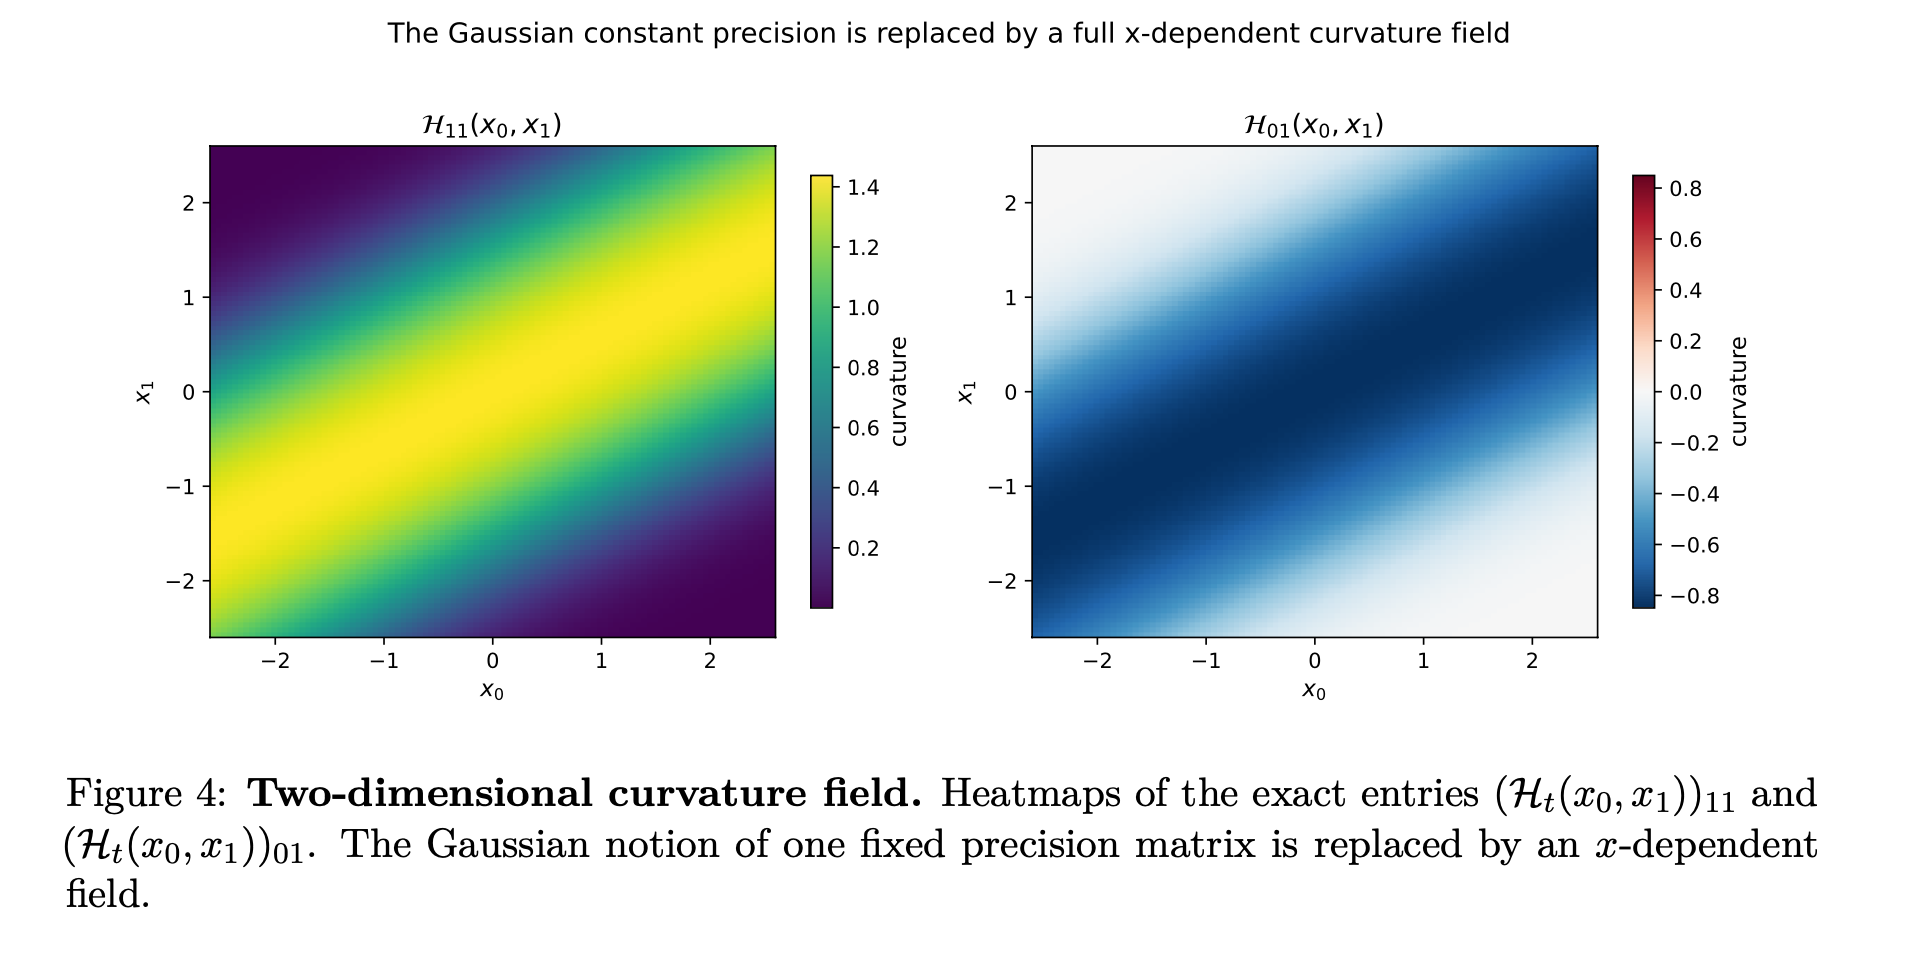
\includegraphics[width=0.98\linewidth]{curvature_field.png}
    \caption{Two entries of the exact curvature field. The visible two-dimensional pattern is entirely generated by the one-dimensional residual variable \(r=x_1-\nu-\rho x_0\). Curvature is concentrated near the residual band \(r\approx 0\), which corresponds approximately to the innovation line \(x_1\approx \alpha x_0\) when \(t\) is small or moderate.}
    \label{fig:curvature-field}
\end{figure}

\subsection{Why the diagonal band appears}

Curvature concentrates where the residual density is most sharply curved, namely around \(r=0\). Therefore the high-curvature region is the straight band
\begin{equation}
\label{eq:residual-band}
x_1 \approx \nu + \rho x_0.
\end{equation}
If \(\mu_0=0\) and \(\Delta\) is not too large, then
\begin{equation}
\rho = \alpha\frac{\beta^2\sigma_0^2}{\beta^2\sigma_0^2+\Delta} \approx \alpha,
\end{equation}
so the band appears visually near the clean innovation line \(x_1\approx \alpha x_0\).

\subsection{Why this is the smoothed remnant of a cusp}

At time \(t=0\), the clean free energy is
\begin{equation}
F_0(x_0,x_1)=\frac{(x_0-\mu_0)^2}{2\sigma_0^2}+\frac{|x_1-\alpha x_0|}{b}+\text{const}.
\end{equation}
The second derivative of \(|u|\) is distributional:
\begin{equation}
\frac{\dd^2}{\dd u^2}|u| = 2\delta(u).
\end{equation}
Therefore the clean curvature is a singular sheet concentrated on the line \(x_1=\alpha x_0\):
\begin{equation}
\curv_0(x)
=
\begin{pmatrix}
\sigma_0^{-2} & 0\\[0.4em]
0 & 0
\end{pmatrix}
+
\frac{2}{b}\delta(x_1-\alpha x_0)
\begin{pmatrix}
\alpha^2 & -\alpha\\[0.3em]
-\alpha & 1
\end{pmatrix}.
\end{equation}
Finite OU smoothing replaces this singular delta-sheet by the smooth diagonal band seen in the figure.

\subsection{Why the off-diagonal entry is negative}

When \(\alpha>0\), one has \(\rho>0\). Moreover the residual density \(h_t\) is log-concave because it is the convolution of two log-concave densities (Gaussian and Laplace). Therefore
\begin{equation}
\kappa_t(r)=-\frac{\dd^2}{\dd r^2}\log h_t(r)\ge 0.
\end{equation}
Hence
\begin{equation}
H_{01}(x)=-\rho\kappa_t(r)\le 0.
\end{equation}
So the off-diagonal field is expected to be negative in the band and to relax toward \(0\) away from it.

\section{Direct answers to the main conceptual questions}

\subsection{Why finite-time OU smoothing does not Gaussianize Laplace}

The reason is exact in Fourier space:
\begin{equation}
\widehat h_t(\ell)=\frac{\exp(-\tau^2\ell^2/2)}{1+\tilde b^2\ell^2}.
\end{equation}
The Gaussian damping factor smooths high frequencies, but the rational Laplace factor remains present for every finite \(t\) because \(\tilde b=\beta b>0\). Therefore higher cumulants do not vanish at finite time. In particular,
\begin{equation}
\kappa_4(R_t)=12\beta^4b^4\neq 0.
\end{equation}
No exact Gaussianization occurs unless \(t\to \infty\).

\subsection{Is the curvature field a local Fisher information?}

Pointwise, \(\curv_t(x)\) is best understood as the Hessian of the free energy or local observed information. After averaging over \(x\), it becomes Fisher information:
\begin{equation}
\E\sq{\curv_t(X)} = \E\sq{\nabla \log \pt(X)\,\nabla \log \pt(X)\trans}.
\end{equation}
So the answer is:
\begin{equation}
\text{pointwise: observed information,}
\qquad
\text{in expectation: Fisher information.}
\end{equation}

\subsection{Is \(\curv_t(x)\) the posterior precision of \(A\given X=x\)?}

Not literally. The exact identity is
\begin{equation}
\curv_t(x)=\frac{1}{\Delta}I - \frac{1}{\Delta^2}\Cov(\beta A\given X=x).
\end{equation}
So \(\curv_t(x)\) is controlled by posterior covariance, not by a latent posterior precision matrix. In the Gaussian case the distinction is less important because Gaussian posteriors are fully described by covariance/precision. In the Laplace case, the posterior is not Gaussian and no single precision matrix captures the whole posterior shape.

\section{Modification guide: what changes when you change the model?}

This section is included so the note can be edited and repurposed easily.

\subsection{Changing the clean innovation law}

If the Laplace innovation is replaced by another centered law with characteristic function \(\widehat f_\varepsilon(\ell)\), then the whole derivation changes only in one place:
\begin{equation}
\widehat h_t(\ell)=\exp(-\tau^2\ell^2/2)\, \widehat f_\varepsilon(\beta \ell).
\end{equation}
Everything else still follows from
\begin{equation}
\pt(x_0,x_1)=\text{Gaussian in }x_0\times h_t(x_1-\nu-\rho x_0).
\end{equation}
So for \(K=1\), many non-Gaussian models remain one-dimensional after conditioning and residualization.

\subsection{Changing \(\alpha\)}

The parameter \(\alpha\) affects
\begin{equation}
\rho=\alpha\frac{\beta^2\sigma_0^2}{v},
\qquad
\nu=\alpha\beta\frac{\Delta\mu_0}{v},
\qquad
\tau^2=\Delta+\alpha^2\beta^2\frac{\sigma_0^2\Delta}{v}.
\end{equation}
So increasing \(|\alpha|\) changes both the orientation of the residual band and the amount of Gaussian broadening in the innovation channel.

\subsection{Changing the prior for \(A_0\)}

The present exact Gaussian formulas for \(m(x_0)\) and \(s^2\) rely on the Gaussian prior for \(A_0\). If that prior changes, then the posterior \(A_0\given X_0\) may cease to be Gaussian, and the residual representation must be modified. In that case, the exact one-dimensional closure may fail, even though the Markov decomposition still gives a local structure.

\section{Compact summary of the main formulas}

For quick reference, here are the main formulas in one place.

\subsection*{Structural constants}
\begin{align}
\beta &= \e^{-t}, & \Delta &= 1-\beta^2, & v &= \beta^2\sigma_0^2+\Delta, \\
\tilde b &= \beta b, & s^2 &= \frac{\sigma_0^2\Delta}{v}, & \tau^2 &= \Delta + \alpha^2\beta^2\frac{\sigma_0^2\Delta}{v}, \\
\rho &= \alpha\frac{\beta^2\sigma_0^2}{v}, & \nu &= \alpha\beta\frac{\Delta\mu_0}{v}, & c &= \frac{\alpha\Delta}{v}.
\end{align}

\subsection*{Residual variable}
\begin{equation}
r=x_1-\nu-\rho x_0 = y+c(x_0-\beta\mu_0),
\qquad y=x_1-\alpha x_0.
\end{equation}

\subsection*{Joint density}
\begin{equation}
\pt(x_0,x_1)=\frac{1}{\sqrt{2\pi v}}\exp\!\left(-\frac{(x_0-\beta\mu_0)^2}{2v}\right) h_t(r).
\end{equation}

\subsection*{Normal--Laplace residual density}
\begin{equation}
h_t(r)=\frac{\exp(a^2/2)}{2\tilde b}
\left[
\exp\!\left(-\frac{r}{\tilde b}\right)\Ph\!\left(\frac{r}{\tau}-a\right)
+
\exp\!\left(\frac{r}{\tilde b}\right)\Ph\!\left(-\frac{r}{\tau}-a\right)
\right],
\qquad a=\frac{\tau}{\tilde b}.
\end{equation}

\subsection*{Score}
\begin{equation}
\score(x,t)=
\begin{pmatrix}
-\dfrac{x_0-\beta\mu_0}{v} - \rho\psi_t(r)\\[0.8em]
\psi_t(r)
\end{pmatrix},
\qquad
\psi_t(r)=\frac{h_t'(r)}{h_t(r)}.
\end{equation}

\subsection*{Curvature}
\begin{equation}
\curv_t(x)=
\begin{pmatrix}
\dfrac{1}{v} & 0\\[0.5em]
0 & 0
\end{pmatrix}
+
\kappa_t(r)
\begin{pmatrix}
\rho^2 & -\rho\\[0.3em]
-\rho & 1
\end{pmatrix},
\qquad
\kappa_t(r)=-\frac{\dd^2}{\dd r^2}\log h_t(r).
\end{equation}

\subsection*{Fourier representation}
\begin{equation}
\widehat p_t(k_0,k_1)
=
\exp\!\left(
\ii\beta\mu_0(k_0+\alpha k_1)
-\frac{\beta^2\sigma_0^2}{2}(k_0+\alpha k_1)^2
-\frac{\Delta}{2}(k_0^2+k_1^2)
\right)
\frac{1}{1+\tilde b^2k_1^2}.
\end{equation}

\section{Closing interpretation}

For \(K=1\), the Laplace AR(1) model under OU corruption is not an arbitrary two-dimensional non-Gaussian problem. It is a one-dimensional non-Gaussian bond attached to a Gaussian site mode. All nonlinear score effects, all curvature variations, and all deviations from the Gaussian benchmark are carried by the single residual coordinate
\begin{equation}
r=x_1-\nu-\rho x_0.
\end{equation}

That is why the heatmaps are so structured: they are not generic two-dimensional landscapes but one-dimensional profiles lifted along straight residual bands. This is the precise sense in which Markovianity creates locality and Laplace innovations create nonlinear bond geometry.

\end{document}
